% sections/model_selection.tex

\section{Semantic Model Selection}
\label{sec:model_selection}

The core routing innovation is \emph{semantic model selection}: once the decision engine matches a routing decision $d^*$, the system analyzes the request's semantic content---its embedding, domain, complexity, and interaction history---to select the most cost-effective model from the decision's candidate set.
Unlike static routing or single-criterion difficulty classifiers, semantic selection operates over the full signal context produced by the signal engine, enabling cost-quality optimization that respects per-decision privacy and safety constraints.

We integrate thirteen algorithms within a unified interface, enabling systematic comparison and hybrid combinations across deployment scenarios.

\subsection{Problem Setting}

Given query embedding $\mathbf{e}_q \in \mathbb{R}^d$, domain category $z \in \{1, \ldots, C\}$, candidate models $\mathcal{M}_{d^*} = \{m_1, \ldots, m_K\}$ with associated costs $\{c_1, \ldots, c_K\}$, and quality estimators, the semantic selection problem is:
\begin{equation}
  m^* = \arg\max_{m_k \in \mathcal{M}_{d^*}} \; \text{Quality}(\mathbf{e}_q, z, m_k; \Theta) - \lambda \cdot \text{Cost}(m_k)
\end{equation}
where $\lambda \geq 0$ is a cost-sensitivity parameter and $\Theta$ represents algorithm-specific parameters.
The per-decision candidate set $\mathcal{M}_{d^*}$ is critical: privacy-constrained decisions restrict candidates to compliant models, while cost-optimized decisions include a broader pool with aggressive cost weighting.
We categorize algorithms into families based on their selection mechanism (\Cref{fig:selection_taxonomy}).

\begin{figure}[t]
\centering
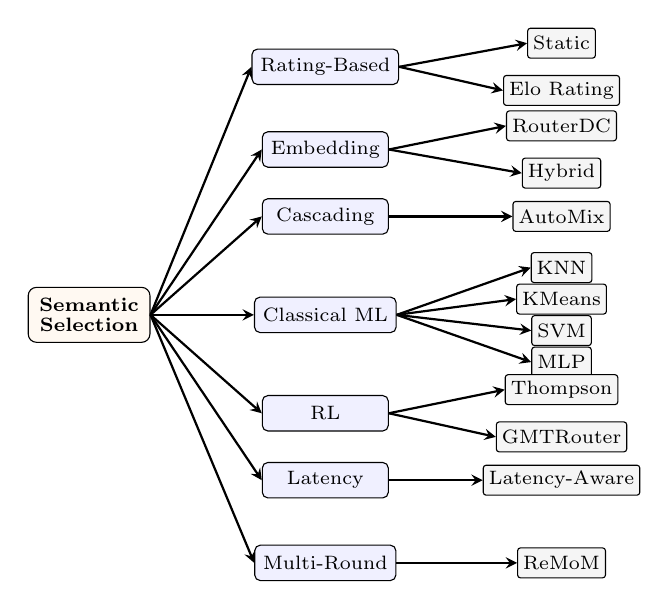
\begin{tikzpicture}[
    node distance=0.2cm,
    fam/.style={rectangle, draw, rounded corners=2pt, fill=blue!6,
                minimum height=0.45cm, minimum width=1.6cm,
                align=left, font=\scriptsize, inner sep=3pt},
    alg/.style={rectangle, draw, rounded corners=1pt, fill=black!4,
                minimum height=0.38cm, align=left,
                font=\scriptsize, inner sep=2pt},
    root/.style={rectangle, draw, rounded corners=3pt, fill=orange!5,
                 minimum height=0.5cm, align=center,
                 font=\scriptsize\bfseries, inner sep=4pt},
    edge from parent/.style={draw, thick, ->, >=stealth},
    level 1/.style={sibling distance=1.05cm, level distance=2.6cm},
  ]
  % Root
  \node[root] (rt) at (0, 0) {Semantic\\[-1pt]Selection};

  % Families (y positions)
  \node[fam] (f1) at (3.0, 3.15) {Rating-Based};
  \node[fam] (f2) at (3.0, 2.1) {Embedding};
  \node[fam] (f3) at (3.0, 1.25) {Cascading};
  \node[fam] (f4) at (3.0, 0.0) {Classical ML};
  \node[fam] (f5) at (3.0, -1.25) {RL};
  \node[fam] (f6) at (3.0, -2.1) {Latency};
  \node[fam] (f7) at (3.0, -3.15) {Multi-Round};

  % Algorithms
  \node[alg] (a1) at (6.0, 3.45) {Static};
  \node[alg] (a2) at (6.0, 2.85) {Elo Rating};
  \node[alg] (a3) at (6.0, 2.4) {RouterDC};
  \node[alg] (a4) at (6.0, 1.8) {Hybrid};
  \node[alg] (a5) at (6.0, 1.25) {AutoMix};
  \node[alg] (a6) at (6.0, 0.6) {KNN};
  \node[alg] (a7) at (6.0, 0.2) {KMeans};
  \node[alg] (a8) at (6.0, -0.2) {SVM};
  \node[alg] (a9) at (6.0, -0.6) {MLP};
  \node[alg] (a10) at (6.0, -0.95) {Thompson};
  \node[alg] (a11) at (6.0, -1.55) {GMTRouter};
  \node[alg] (a12) at (6.0, -2.1) {Latency-Aware};
  \node[alg] (a13) at (6.0, -3.15) {ReMoM};

  % Root → Families
  \foreach \f in {f1,f2,f3,f4,f5,f6,f7}
    \draw[thick, ->, >=stealth] (rt.east) -- (\f.west);

  % Families → Algorithms
  \draw[thick, ->, >=stealth] (f1.east) -- (a1.west);
  \draw[thick, ->, >=stealth] (f1.east) -- (a2.west);
  \draw[thick, ->, >=stealth] (f2.east) -- (a3.west);
  \draw[thick, ->, >=stealth] (f2.east) -- (a4.west);
  \draw[thick, ->, >=stealth] (f3.east) -- (a5.west);
  \draw[thick, ->, >=stealth] (f4.east) -- (a6.west);
  \draw[thick, ->, >=stealth] (f4.east) -- (a7.west);
  \draw[thick, ->, >=stealth] (f4.east) -- (a8.west);
  \draw[thick, ->, >=stealth] (f4.east) -- (a9.west);
  \draw[thick, ->, >=stealth] (f5.east) -- (a10.west);
  \draw[thick, ->, >=stealth] (f5.east) -- (a11.west);
  \draw[thick, ->, >=stealth] (f6.east) -- (a12.west);
  \draw[thick, ->, >=stealth] (f7.east) -- (a13.west);
\end{tikzpicture}
\caption{Taxonomy of thirteen semantic model selection algorithms organized by selection mechanism.  Families span from lightweight rating-based methods (Static, Elo) to learned approaches (RouterDC, Classical ML, RL), adaptive cascading (AutoMix), real-time latency tracking, and multi-round synthesis (ReMoM).}
\label{fig:selection_taxonomy}
\end{figure}

\subsection{Rating-Based Selection}

\noindent\textbf{Static.}
Each model carries a pre-configured quality score $s_k$; selection is $m^* = \arg\max_k s_k$.
Serves as a deterministic baseline.

\noindent\textbf{Elo Rating} (adapted from RouteLLM~\cite{ong2024routellm}).
Models maintain Elo ratings $R_k$ updated from pairwise user preference feedback.
Selection probability follows the Bradley-Terry model:
\begin{equation}
  P(m_i \succ m_j) = \frac{1}{1 + 10^{(R_j - R_i)/400}}
\end{equation}
Models are sampled proportional to their expected win rate against the candidate pool.
Ratings are updated online as user feedback arrives.

\subsection{Embedding-Based Selection}

\noindent\textbf{RouterDC}~\cite{chen2024routerdc}.
Dual contrastive learning trains query and model encoders to produce embeddings in a shared space.
Selection maximizes cosine similarity:
\begin{equation}
  m^* = \arg\max_{m_k \in \mathcal{M}_{d^*}} \cos(\mathbf{e}_q, \mathbf{e}_{m_k})
\end{equation}
The contrastive training objective encourages queries to be close to their best-performing model's embedding and distant from poorly-performing models.

\noindent\textbf{Hybrid}~\cite{hu2024routerbench}.
Combines Elo ratings, embedding similarity, and cost in a weighted score:
\begin{equation}
  \text{score}(m_k) = \alpha \cdot \tilde{R}_k + \beta \cdot \cos(\mathbf{e}_q, \mathbf{e}_{m_k}) + \gamma \cdot (1 - \tilde{c}_k)
\end{equation}
where $\tilde{R}_k$ and $\tilde{c}_k$ are normalized ratings and costs, and $\alpha + \beta + \gamma = 1$ are configurable weights.

\subsection{Cascading Selection}

\noindent\textbf{AutoMix}~\cite{aggarwal2023automix}.
Formulated as a Partially Observable Markov Decision Process (POMDP).
Models are ordered by capability $m_1 \prec m_2 \prec \cdots \prec m_K$.
The cascade:
\begin{enumerate}
  \item Generate response $a_k$ with current model $m_k$ (starting from $k=1$, the cheapest).
  \item Self-verify: estimate response quality $\hat{q}_k$ using $m_k$ itself.
  \item If $\hat{q}_k \geq \tau_k$, accept $a_k$; otherwise, escalate to $m_{k+1}$.
\end{enumerate}
The expected cost is:
\begin{equation}
  \mathbb{E}[C] = \sum_{k=1}^{K} C_k \cdot \prod_{j=1}^{k-1}(1 - P(\hat{q}_j \geq \tau_j))
\end{equation}
where $P(\hat{q}_j \geq \tau_j)$ is the probability that model $m_j$ passes self-verification.
This naturally trades off cost against quality.

\subsection{Classical ML Selection}

These methods train on routing records $\{(\mathbf{e}_q^{(i)}, z^{(i)}, m^{*(i)}, q^{(i)})\}$ where $q^{(i)}$ is a quality score.
Feature vectors combine embeddings and domain information:
\begin{equation}
  \mathbf{f} = [\mathbf{e}_q \in \mathbb{R}^d; \; \text{onehot}(z) \in \{0,1\}^C]
\end{equation}

\noindent\textbf{KNN.}
$k$-nearest neighbor search with Ball Tree indexing.
Quality-weighted majority voting:
\begin{equation}
  m^* = \arg\max_m \sum_{i \in \text{kNN}(\mathbf{f})} \mathbf{1}[m^{*(i)} = m] \cdot q^{(i)}
\end{equation}

\noindent\textbf{KMeans.}
Assigns queries to pre-computed clusters; selects the best model for the assigned cluster based on a combined quality-latency score:
\begin{equation}
  m^* = \arg\max_m \bigl(\alpha \cdot \text{quality}(m, z_\text{cluster}) - (1-\alpha) \cdot \text{latency}(m)\bigr)
\end{equation}

\noindent\textbf{SVM.}
Multi-class SVM with RBF or linear kernel, trained to classify feature vectors directly into model selections.

\noindent\textbf{MLP.}
A feed-forward neural network (two hidden layers with ReLU activation) mapping $\mathbf{f}$ to a softmax distribution over candidate models:
\begin{equation}
  P(m_k \mid \mathbf{f}) = \text{softmax}\bigl(W_2 \cdot \text{ReLU}(W_1 \mathbf{f} + b_1) + b_2\bigr)_k
\end{equation}
The MLP is implemented in the GPU-accelerated Candle runtime for low-latency inference.

\subsection{Reinforcement Learning Selection}

\noindent\textbf{Thompson Sampling}~\cite{thompson1933likelihood}.
Each model maintains a Beta prior:
\begin{equation}
  \theta_k \sim \text{Beta}(\alpha_k, \beta_k)
\end{equation}
Selection samples from each posterior and picks the maximum: $m^* = \arg\max_k \theta_k$.
Parameters $(\alpha_k, \beta_k)$ are updated from user preference feedback, naturally balancing exploration and exploitation.

\noindent\textbf{GMTRouter}~\cite{xie2025gmtrouter}.
Models multi-turn user-query-model interactions as a heterogeneous graph.
Graph neural network message passing captures complex interaction patterns:
\begin{equation}
  \mathbf{h}_v^{(l+1)} = \text{AGG}\bigl(\{\mathbf{h}_u^{(l)} \mid u \in \mathcal{N}(v)\}\bigr)
\end{equation}
where nodes represent users, queries, and models, and edges encode historical routing outcomes.

\subsection{Latency-Aware Selection}

\noindent\textbf{Latency-Aware.}
Selects the model with the best observed latency using percentile-based Time-per-Output-Token (TPOT) and Time-to-First-Token (TTFT) statistics collected at runtime.
For each candidate model $m_k$, the selector computes a normalized latency score:
\begin{equation}
  s_k = \frac{1}{|P|} \sum_{p \in P} \frac{\text{perc}_p(m_k)}{\min_{j}\, \text{perc}_p(m_j)}
\end{equation}
where $P \subseteq \{\text{TPOT}, \text{TTFT}\}$ is the set of configured performance metrics and $\text{perc}_p(m_k)$ is the observed percentile value for model $m_k$ on metric $p$.
Selection minimizes this score: $m^* = \arg\min_k s_k$.
This enables adaptive routing that responds to real-time backend performance degradation without requiring explicit latency thresholds as signal conditions.

\subsection{Multi-Round Reasoning (ReMoM)}

The ReMoM (Reasoning for Mixture of Models) strategy extends single-shot selection to multi-round parallel reasoning with LLM-driven synthesis.
Inspired by PaCoRe~\cite{pacore2025} but generalized to heterogeneous model pools, ReMoM executes a \emph{breadth schedule} of decreasing parallelism across rounds, where each subsequent round synthesizes the outputs of the previous round via prompted LLM calls (\Cref{fig:remom_flow}).

\begin{figure}[t]
\centering
\begin{tikzpicture}[
    node distance=0.3cm,
    call/.style={rectangle, draw, rounded corners=2pt,
                 minimum height=0.48cm, minimum width=1.35cm,
                 align=center, font=\scriptsize, inner sep=2pt},
    synth/.style={trapezium, draw, trapezium angle=75, rounded corners=1pt,
                  fill=orange!8, minimum height=0.5cm,
                  align=center, font=\scriptsize, inner sep=3pt},
    query/.style={rectangle, draw, rounded corners=2pt, fill=black!4,
                  font=\scriptsize, inner sep=3pt, align=center},
    outbox/.style={rectangle, draw, rounded corners=3pt, fill=green!8,
                   font=\scriptsize\bfseries, inner sep=4pt, align=center},
    roundlbl/.style={font=\scriptsize\bfseries, text=gray!70},
    arr/.style={->, >=stealth, thick},
    arrs/.style={->, >=stealth, semithick, gray!60},
  ]

  % === Query ===
  \node[query] (q) at (0, 0) {Query $q$};

  % === Round 1: b_1 = 4 ===
  \node[roundlbl] at (2.5, 1.55) {Round 1 ($b_1{=}4$)};
  \node[call, fill=blue!10]   (r1c1) at (2.5, 1.0)  {\footnotesize $m_A$};
  \node[call, fill=blue!10]   (r1c2) at (2.5, 0.4)  {\footnotesize $m_B$};
  \node[call, fill=blue!10]   (r1c3) at (2.5, -0.2) {\footnotesize $m_A$};
  \node[call, fill=yellow!15] (r1c4) at (2.5, -0.8) {\footnotesize $m_C$};

  % Parallel bracket
  \draw[decorate, decoration={brace, amplitude=4pt, mirror}, thick, gray!50]
    (1.7, 1.25) -- (1.7, -1.05) node[midway, left=5pt, font=\tiny, text=gray] {parallel};

  % Query → Round 1
  \draw[arr] (q.east) -- ++(0.4,0) |- (r1c1.west);
  \draw[arr] (q.east) -- ++(0.4,0) |- (r1c2.west);
  \draw[arr] (q.east) -- ++(0.4,0) |- (r1c3.west);
  \draw[arr] (q.east) -- ++(0.4,0) |- (r1c4.west);

  % === Synthesis 1 ===
  \node[synth] (s1) at (4.7, 0.1) {Synthesis\\[-1pt]Prompt};

  % Round 1 → Synthesis 1
  \draw[arrs] (r1c1.east) -- ++(0.3,0) |- (s1.west);
  \draw[arrs] (r1c2.east) -- (s1.west);
  \draw[arrs] (r1c3.east) -- ++(0.3,0) |- (s1.west);
  \draw[arrs] (r1c4.east) -- ++(0.3,0) |- (s1.west);

  % === Round 2: b_2 = 2 ===
  \node[roundlbl] at (6.8, 0.95) {Round 2 ($b_2{=}2$)};
  \node[call, fill=blue!10]   (r2c1) at (6.8, 0.4)  {\footnotesize $m_B$};
  \node[call, fill=yellow!15] (r2c2) at (6.8, -0.2) {\footnotesize $m_C$};

  % Synthesis 1 → Round 2
  \draw[arr] (s1.east) -- ++(0.2,0) |- (r2c1.west);
  \draw[arr] (s1.east) -- ++(0.2,0) |- (r2c2.west);

  % === Synthesis 2 ===
  \node[synth] (s2) at (8.8, 0.1) {Synthesis\\[-1pt]Prompt};

  % Round 2 → Synthesis 2
  \draw[arrs] (r2c1.east) -- ++(0.15,0) |- (s2.west);
  \draw[arrs] (r2c2.east) -- ++(0.15,0) |- (s2.west);

  % === Round 3: b_3 = 1 (final) ===
  \node[roundlbl] at (10.7, 0.55) {Final ($b_3{=}1$)};
  \node[call, fill=blue!10] (r3c1) at (10.7, 0.1) {\footnotesize $m_A$};

  % Synthesis 2 → Round 3
  \draw[arr] (s2.east) -- (r3c1.west);

  % === Output ===
  \node[outbox] (out) at (12.6, 0.1) {Output};
  \draw[arr] (r3c1.east) -- (out.west);

  % === Compaction annotation ===
  \node[font=\tiny, text=gray, anchor=north] at (4.7, -1.25)
    {optionally compact responses};
  \draw[densely dotted, gray!40] (4.7, -1.15) -- (s1.south);
  \draw[densely dotted, gray!40] (8.8, -1.15) -- (s2.south);
  \node[font=\tiny, text=gray, anchor=north] at (8.8, -1.25)
    {before prompt construction};

\end{tikzpicture}
\caption{ReMoM execution flow with breadth schedule $\mathbf{b} = [4, 2]$.
Round~1 distributes 4~parallel calls across models ($m_A$, $m_B$, $m_C$); responses are (optionally compacted and) assembled into a synthesis prompt.
Round~2 sends 2~parallel synthesis calls.
A final round ($b_3 = 1$, auto-appended) produces the single output.
Each synthesis prompt includes the original query and all previous-round responses as numbered references, delegating quality judgment to the synthesizing LLM.}
\label{fig:remom_flow}
\end{figure}

\noindent\textbf{Breadth schedule.}
The operator specifies a breadth schedule $\mathbf{b} = [b_1, b_2, \ldots, b_R]$ defining the number of parallel model calls per round.
A final synthesis round with $b_{R+1} = 1$ is automatically appended, yielding a total of $R+1$ rounds.
For example, $\mathbf{b} = [32, 4]$ produces three rounds: 32 parallel calls, then 4 parallel calls each synthesizing the 32 responses, then a single final call synthesizing the 4 responses.

\noindent\textbf{Model distribution.}
At each round, $b_r$ calls are distributed among the candidate models $\mathcal{M}_{d^*}$ according to one of three strategies:
(1)~\emph{equal}: calls are distributed evenly across all candidates with round-robin remainder allocation;
(2)~\emph{weighted}: calls are distributed proportionally to model weights (currently equivalent to equal distribution);
(3)~\emph{first\_only}: all $b_r$ calls target a single model with different random seeds, providing PaCoRe-compatible single-model diversity.
Calls within each round execute concurrently with configurable concurrency limits.

\noindent\textbf{LLM-driven synthesis.}
After collecting responses from round $r$, the system constructs a synthesis prompt for round $r+1$ using a configurable Go \texttt{text/template}.
The default template presents the original query alongside all previous-round responses as numbered references, instructing the next-round model(s) to \emph{``analyze these references and provide your own comprehensive solution.''}
When reasoning content is available (e.g., from models supporting extended thinking), the template additionally includes each reference's chain-of-thought reasoning.
This approach delegates quality judgment entirely to the synthesizing LLM rather than relying on explicit scoring or weighted aggregation.

\noindent\textbf{Response compaction.}
To manage prompt length across rounds, responses can be compacted before inclusion in synthesis prompts.
Two strategies are supported: \emph{full} (no compaction, the default) and \emph{last\_n\_tokens} (retaining only the final $N$ tokens, estimated at $\sim$4 characters per token).
This is particularly important for high-breadth schedules where concatenating all responses would exceed context limits.

\noindent\textbf{Execution flow.}
The complete algorithm proceeds as:
\begin{enumerate}
  \item \textbf{Schedule construction}: Append $[1]$ to the user-specified breadth schedule $\mathbf{b}$.
  \item \textbf{Round~1 (parallel generation)}: Distribute $b_1$ calls across candidate models; execute concurrently with temperature $T$ (default 1.0) for response diversity.
  \item \textbf{Rounds~$2 \ldots R{+}1$ (synthesis)}: For each subsequent round, build a synthesis prompt from the previous round's (optionally compacted) responses, distribute $b_r$ calls, and execute concurrently.
  \item \textbf{Final output}: Return the single response from the final round ($b_{R+1} = 1$).
\end{enumerate}

ReMoM is particularly effective when model capabilities are uncertain or when the task benefits from diverse perspectives (e.g., complex reasoning, multi-faceted analysis).
The breadth schedule provides fine-grained control over the cost--quality tradeoff: higher initial breadth increases diversity at the cost of additional LLM calls, while the funneling structure ensures convergence to a single synthesized answer.

\subsection{Unified Selection Interface}

All thirteen algorithms implement a common interface:
\begin{equation}
  \text{Select}: (\mathbf{e}_q, z, \mathcal{M}, \Theta) \to (m^*, c)
\end{equation}
returning the selected model and a confidence score.
This uniformity enables:
(1)~per-decision algorithm selection---different routing decisions can use different selection algorithms, allowing cost-optimized decisions to use cascading (AutoMix) while quality-sensitive decisions use embedding-based (RouterDC) selection;
(2)~A/B testing across algorithms on live traffic;
(3)~ensemble methods that combine multiple selectors.

\subsection{Cost-Aware Selection in Multi-Provider Settings}

In multi-endpoint deployments where the same logical model may be served by different providers at different price points, the selection algorithms operate in conjunction with the endpoint router (\Cref{subsec:multi_endpoint}).
The selection algorithm chooses the best \emph{model} based on semantic analysis, and the endpoint router resolves it to the most cost-effective \emph{provider endpoint}.
This two-stage process separates quality optimization (which model is best for this query?) from cost optimization (which provider endpoint offers the best price for this model?), enabling fine-grained cost management across heterogeneous multi-cloud deployments.
